% Research paper draft. Compile on Overleaf: pdfLaTeX, then BibTeX, then pdfLaTeX twice.
\documentclass[journal]{IEEEtran}

\usepackage[utf8]{inputenc}
\usepackage[T1]{fontenc}
\usepackage{cite}
\usepackage{graphicx}
\usepackage{booktabs}
\usepackage{tabularx}
\usepackage{array}
\usepackage{url}
\usepackage{amsmath}
\usepackage{xcolor}
\usepackage[hidelinks]{hyperref}

\graphicspath{{figures/}}
\newcolumntype{Y}{>{\raggedright\arraybackslash}X}
\newcolumntype{L}[1]{>{\raggedright\arraybackslash}p{#1}}
% Visible reminders for the team. Search for \todo before submitting.
\newcommand{\todo}[1]{\textcolor{red}{[#1]}}

\begin{document}

\title{When Does Online Alignment Help EEG Drowsiness Detection? State Mix, Reference Stability and Explanations on Real Drives}

\author{Sunny Yadav, Akshay \todo{surname}, Aryan \todo{surname}, and Prachi \todo{surname}%
\thanks{The authors are with the Indian Institute of Technology Roorkee, India. \todo{department, supervisor, e-mail}}}

\maketitle

\begin{abstract}
A drowsiness detector in a vehicle must work on a new driver without a calibration session. Online Euclidean alignment offers this, and it is now being used in electroencephalography (EEG) test-time adaptation, but its behaviour during a real drive is poorly understood. Using all 62 sessions from 27 drivers of a public lane-keeping dataset under leave-one-subject-out testing, we examine when it helps. Short references are near-singular in every session and collapse accuracy to 52.55\%; shrinkage restores it to 74.79\%. Blending the running covariance with a population prior raises balanced accuracy from 73.59\% to 77.37\% ($p = 0.039$), matching whole-session alignment, although the result depends on a few drivers and AUC does not improve. Exploratory analysis shows the gain varies with the drowsy share of windows seen so far: about one point at low share, 7.70 and 12.47 points in the middle bins, and about one point above 75\%. This pattern is entangled with time on task. A frozen early reference loses 6.40 points late in the drive. Updating batch-normalisation statistics during the drive harms this model, lowering accuracy to 53.84\% at a published setting. Alignment also increases reliance on gamma and theta activity and weakens attribution tests. These results come from one model and one dataset, but they suggest that the mix of states in the reference, not only its length, should guide online EEG adaptation.
\end{abstract}

\begin{IEEEkeywords}
Drowsiness detection, electroencephalography, Euclidean alignment, test-time adaptation, batch normalisation, cross-subject, explainability.
\end{IEEEkeywords}

\section{Introduction}
\IEEEPARstart{E}{EG} models for drowsiness detection lose accuracy on drivers they have not seen, and a vehicle cannot ask each new driver for a labelled calibration session. Euclidean alignment (EA) \cite{he2020transfer} reduces this gap without labels by whitening each person's EEG with their own mean covariance. The difficulty is that this mean normally needs the whole session, which does not exist yet during a drive.

Recent work therefore updates the reference online. Duan \textit{et al.}~\cite{duan2025online} blend a training reference with incoming trials for motor imagery and SSVEP, and Li \textit{et al.}~\cite{li2026backprop} include online EA and batch-norm adaptation in test-time methods evaluated on drowsiness regression. We do not propose a new alignment method. We ask a question specific to drowsiness that we did not find addressed in the literature we searched: \textit{when does online alignment help during a real drive, and why?}

Drowsiness makes this question distinctive. In motor imagery, classes alternate quickly, so a short reference tends to contain all of them. In a drive, the state changes slowly, so a reference early in a session may contain almost only alert windows. Gao and Lv \cite{gao2026early} freeze an early reference to keep late fatigue out of it. Our earlier experiments on the 11-subject subset suggested the opposite: the gain from alignment was largest for mixed-state references.

We study this on all 27 drivers and 62 sessions of the Cao \textit{et al.} dataset \cite{cao2019multichannel}, in time order, under leave-one-subject-out (LOSO) testing. Our contributions are:
\begin{enumerate}
\item an exploratory analysis showing, on real drives, that the gain from online alignment varies with the state mix seen so far;
\item evidence that a running reference holds up late in a drive where a frozen early one does not;
\item a diagnosis of why short references fail on this data, and how shrinkage or a population prior prevents it;
\item evidence that updating batch-norm statistics during a drive can severely harm a model that decides from pooled activations; and
\item tests of how alignment changes what the model relies on and how well attributions hold up.
\end{enumerate}

\section{Related Work}
\label{sec:related}

\textit{Alignment.} EA \cite{he2020transfer} and Riemannian re-centring \cite{zanini2018transfer} are standard for cross-subject EEG; Wu \cite{wu2025revisiting} and Junqueira \textit{et al.}~\cite{junqueira2024systematic} evaluate EA more broadly. Our population-prior reference has essentially the same form as Equation 8 of Duan \textit{et al.}~\cite{duan2025online}, so we treat it as an existing method applied to a new setting. Chu \textit{et al.}~\cite{chu2026rectifying} address class imbalance in online re-centring, but on motor imagery with simulated imbalance, and latent alignment has been examined under imbalance on other EEG tasks \cite{latent2025}. \todo{Team: confirm these two descriptions from the full papers.}

\textit{Test-time adaptation.} Wimpff \textit{et al.}~\cite{wimpff2023calibration} combine alignment and batch-norm updates for motor imagery. Li \textit{et al.}~\cite{li2026backprop} use online EA and batch-norm adaptation within forward-only adaptation for drowsiness regression; they describe both as effective tools and do not analyse the reference's state mix. For drowsiness classification, Jang \textit{et al.}~\cite{jang2025calibration} adapt online while keeping pretrained batch-norm statistics.

\textit{Calibration-free drowsiness detection.} Other work approaches this problem through domain generalisation \cite{dg2023,manifold2024}, black-box adaptation \cite{spark2024} and cross-dataset transfer \cite{edjan2023}. Gao and Lv \cite{gao2026early} use a frozen personal spectral reference from the session's opening and find that even very short windows suffice, under a different feature space and label scheme from ours. Our base model is InterpretableCNN \cite{cui2022eeg}.

\textit{Explanations.} Attribution methods on EEG vary in faithfulness \cite{cui2023towards}, and few drowsiness studies test them. We did not find a study of how online alignment changes attributions for drowsiness.

\section{Data and Methods}
\label{sec:methods}

\subsection{Data and labels}
The Cao \textit{et al.} dataset \cite{cao2019multichannel} contains 62 sessions from 27 subjects performing a 90-minute lane-keeping task in a virtual-reality simulator, with random lane departures. We used the pre-processed 30-channel release. Each trial is the 3 s before a deviation onset, resampled to 128 Hz, kept in time order. Reaction time (RT) defines the labels, following Cui \textit{et al.}~\cite{cui2022eeg}: with alert RT as the 5th percentile of a session's valid RTs, a trial is alert if its RT and the mean RT of the preceding 90 s are both below 1.5 times alert RT, drowsy if both exceed 2.5 times, and unlabelled otherwise. Trials with RT below 0.3 s were rejected as artefacts, following the dataset's tutorial. This gave 27{,}192 trials: 8{,}941 alert and 3{,}947 drowsy, with the rest unlabelled or invalid. Unlike studies that keep one session per subject, we use every session and the natural class balance.

\subsection{Protocol}
All experiments use LOSO over 27 subjects and five seeds, with InterpretableCNN \cite{cui2022eeg} trained for a fixed 11 epochs (Adam, learning rate 0.001, batch 50), so no test data select the training length. Models use running batch-norm statistics, so a window can be scored alone. Training uses the labelled trials of the other subjects. Unless stated, scoring covers labelled trials from the 31st of each session, the same trials for every method. The primary metric is balanced accuracy, reported with AUC. Comparisons use two-sided Wilcoxon signed-rank tests across subjects, on per-subject means over seeds.

\subsection{Alignment}
Training subjects are whitened per session with their whole-session reference, which is available offline. A held-out window $x$ is transformed to $R^{-1/2}x$, with $R$ a mean of sample covariances. We compare a fixed reference from the first 30 windows; a cumulative reference of all windows so far; the last 100 windows; and the whole session, which is not available live but serves as a reference point. All references are label-free and causal, except the whole-session one.

Two forms of regularisation are tested. \textit{Shrinkage} replaces every reference, in training too, with $(1-\alpha)R + \alpha\,\mathrm{tr}(R)/C \cdot I$. We report $\alpha = 0.1$, chosen by inspecting seed 0 of the same test subjects from 0.01, 0.05, 0.1 and 0.2; on that seed, cumulative alignment ranged from 75.34\% to 76.02\% across these values, so the choice adds little tuning gain. The \textit{population prior} uses
\begin{equation}
R_t = (n\,\hat{R}_t + \kappa\,R_{\mathrm{pop}})/(n + \kappa),
\end{equation}
where $\hat{R}_t$ is the session's running mean, $n$ the windows seen so far, and $R_{\mathrm{pop}}$ the mean covariance of the training subjects, recomputed in each fold. This has essentially the same form as Duan \textit{et al.}~\cite{duan2025online}. We fixed $\kappa = 30$ against no alignment as the primary test before seeing results, with $\kappa = 10$ and 100 as sensitivity checks, and $R_{\mathrm{pop}}$ alone as a control that uses no data from the driver.

\subsection{Batch-norm adaptation}
We tested online updates of the statistics of the batch-norm layer, causally, without alignment and on top of it: a blend of training statistics and the session so far, with weight 10, 30 or 100; and an exponential moving average with weight 0.1 or 0.7 on the current trial, the latter being the setting of Duan \textit{et al.}~\cite{duan2025online}, whose self-supervised loss we did not reproduce. The prespecified tests were prior alignment against blended adaptation with weight 30 and, separately, prior alignment with and without the 0.7 update. These are our own implementations.

\subsection{State-mix analysis}
Each scored trial is assigned the share of drowsy trials among labelled trials so far in its session, and placed in one of five bins. Labels are used only for this analysis. Gain is balanced accuracy minus that of no alignment, paired per subject, counting a subject in a bin only if both classes occur there. This analysis was not prespecified as a primary test.

\subsection{Explanation tests}
We compared unaligned and prior-aligned models on saliency and gradient$\times$input, computed with respect to the raw input through the fixed per-window whitener so channels remain comparable. Tests were point and channel deletion against a random baseline; a sanity check \cite{adebayo2018sanity} against a re-initialised model; and removal of each frequency band and of the 15 peripheral or 15 central channels, with six prior-versus-none comparisons fixed in advance and Holm-corrected.

\section{Results}
\label{sec:results}

\subsection{Short references and their fix}
The first-30 reference had a condition number above $10^{10}$ in all 62 sessions (median about $3 \times 10^{14}$), against about $5 \times 10^{3}$ for whole-session references in the median. The pre-processed EEG is rank-deficient, and the null directions appear to change over a session, so a short average leaves near-zero eigenvalues that amplify later signal. Accuracy collapsed accordingly (Table~\ref{tab:main}; AUC 0.533). Shrinkage at $\alpha = 0.1$ brought the condition number to about 150 and restored accuracy to 74.79\%.

\begin{table}[!t]
\centering
\caption{Online Alignment on 27 Subjects, Five Seeds. Trials from the 31st of Each Session; $\Delta$ and $p$ Against No Alignment}
\label{tab:main}
\footnotesize
\setlength{\tabcolsep}{3pt}
\begin{tabularx}{\columnwidth}{@{}YL{0.8cm}L{0.8cm}L{0.75cm}L{0.8cm}L{0.8cm}@{}}
\toprule
\textbf{Method} & \textbf{Bal. acc.} & \textbf{$\Delta$} & \textbf{W/L} & \textbf{$p$} & \textbf{AUC} \\
\midrule
No alignment & 73.59 & -- & -- & -- & 0.828 \\
\midrule
\multicolumn{6}{@{}l}{\textit{No regularisation}} \\
First 30 & 52.55 & $-21.04$ & 3/24 & $<$0.001 & 0.533 \\
Cumulative & 75.26 & $+1.67$ & 13/14 & 0.66 & 0.802 \\
Last 100 & 71.76 & $-1.83$ & 8/19 & 0.17 & 0.765 \\
Whole session & 77.85 & $+4.26$ & 19/8 & 0.019 & 0.834 \\
\midrule
\multicolumn{6}{@{}l}{\textit{Shrinkage, $\alpha = 0.1$}} \\
First 30 & 74.79 & $+1.20$ & 14/13 & 0.55 & 0.801 \\
Cumulative & 76.25 & $+2.66$ & 16/11 & 0.155 & 0.818 \\
Last 100 & 74.77 & $+1.18$ & 12/15 & 0.86 & 0.810 \\
Whole session & 77.27 & $+3.68$ & 18/9 & 0.032 & 0.832 \\
\midrule
\multicolumn{6}{@{}l}{\textit{Population prior}} \\
$\kappa = 30$ (primary) & 77.37 & $+3.78$ & 18/9 & 0.039 & 0.820 \\
$\kappa = 10$ & 77.01 & $+3.42$ & 17/10 & 0.065 & 0.817 \\
$\kappa = 100$ & 77.08 & $+3.49$ & 18/9 & 0.032 & 0.820 \\
$R_{\mathrm{pop}}$ only & 74.12 & $+0.53$ & 13/14 & 0.75 & 0.804 \\
\bottomrule
\end{tabularx}
\end{table}

\subsection{Online alignment}
The prespecified test favoured the prior: $+3.78$ points against no alignment (18/9 subjects, $p = 0.039$). It showed no detectable loss against whole-session alignment without shrinkage ($-0.48$, $p = 0.90$). The result is sensitive to a few drivers: the median gain is 2.41 points, and removing the subject with the largest gain (34.3 points) gives $+2.60$ ($p = 0.067$). AUC did not improve ($-0.009$, $p = 0.46$), so the gain looks like better threshold calibration for a new driver, not better ranking; whole-session alignment shows the same pattern. The prior was not significantly better than shrunk cumulative alignment ($+1.11$, $p = 0.20$). The prior alone gave no gain, and the full method beat it ($+3.25$, 20/7, $p = 0.013$, not prespecified), so the benefit comes from the driver's own data.

\subsection{Time course}
Fig.~\ref{fig:time} shows when the gain arrives. It is absent early: the prior gains $+0.18$ points in trials 31--100, and $-3.72$ on the first 30 trials (10 subjects, $p = 0.13$), so the prior prevents instability but does not bring an early benefit. Gains appear in the middle of the session ($+5.96$ in trials 201--300, 13/5, $p = 0.0096$). A frozen first-30 reference loses 6.40 points after trial 300 (2/13, $p = 0.0015$). Across all scored trials, the running prior beat the frozen reference by 2.57 points (18/9, $p = 0.08$), although the two used different training regularisation. These bins are exploratory and contain different subjects.

\begin{figure}[!t]
\centering
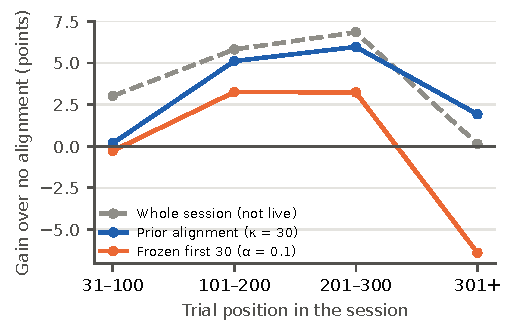
\includegraphics[width=\columnwidth]{fig2_time}
\caption{Gain over no alignment by trial position, five seeds. Each point compares subjects with both classes in that bin; subject sets differ between bins. Exploratory.}
\label{fig:time}
\end{figure}

\subsection{State mix}
Fig.~\ref{fig:statemix} shows the gain by drowsy share so far. For the prior it was $+1.22$ and $+1.24$ points below 25\%, $+7.70$ at 25--50\% (12/4, $p = 0.0076$), $+12.47$ at 50--75\% (8/3, $p = 0.032$) and $+1.18$ above 75\% (2/4, 6 subjects, $p = 1.0$). Shrunk cumulative alignment has the same shape. This resembles our earlier inverted U on the 11-subject subset, where windows were built with fixed mixes, so the pattern appears both with constructed references and on real timelines. Two limits apply. These tests are uncorrected, and the upper bins contain few subjects. More importantly, drowsy share rises with time on task, so we cannot separate state mix from elapsed time here. \todo{Consider the within-time-bin check before submitting.}

\begin{figure}[!t]
\centering
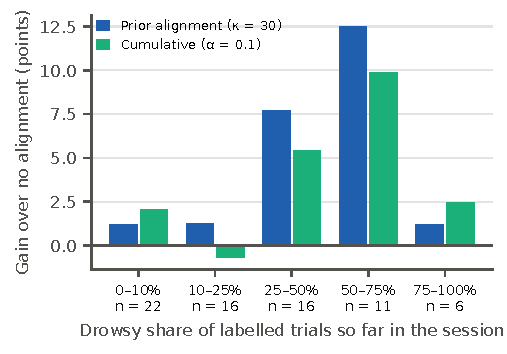
\includegraphics[width=\columnwidth]{fig1_statemix}
\caption{Gain over no alignment by drowsy share of labelled trials so far in the session; $n$ is the number of subjects with both classes in that bin. Exploratory and entangled with time on task.}
\label{fig:statemix}
\end{figure}

\subsection{Batch-norm adaptation}
Table~\ref{tab:bn} shows that updating batch-norm statistics hurt in every setting. The prespecified comparison favoured prior alignment over blended adaptation by 6.81 points (23/4, $p = 0.0008$; AUC difference not significant, $p = 0.19$). Adding the update to prior alignment was worse: at the setting of Duan \textit{et al.}, accuracy fell to 53.84\% (2/25, $p < 0.0001$). The harm grew as the statistics gave more weight to the current window. This model decides from the time-averaged output of its batch-norm layer, so statistics dominated by the current window subtract much of the evidence; we reasoned this from the architecture and did not test it separately. With Riemannian logistic regression, the prior gave no gain ($-0.17$, $p = 0.99$) and AUC fell from 0.739 to 0.701, so the alignment benefit is not model-independent either.

\begin{table}[!t]
\centering
\caption{Batch-Norm Adaptation, Five Seeds. $\Delta$ Against No Alignment (73.59\%)}
\label{tab:bn}
\footnotesize
\setlength{\tabcolsep}{3pt}
\begin{tabularx}{\columnwidth}{@{}YL{0.8cm}L{0.85cm}L{0.7cm}L{0.8cm}@{}}
\toprule
\textbf{Method} & \textbf{Bal. acc.} & \textbf{$\Delta$} & \textbf{W/L} & \textbf{AUC} \\
\midrule
\multicolumn{5}{@{}l}{\textit{Without alignment}} \\
Blend, weight 100 & 71.05 & $-2.54$ & 8/19 & 0.815 \\
Blend, weight 30 & 70.56 & $-3.03$ & 8/19 & 0.802 \\
Blend, weight 10 & 70.09 & $-3.50$ & 9/18 & 0.794 \\
Moving average, 0.1 & 59.58 & $-14.01$ & 3/24 & 0.651 \\
\midrule
\multicolumn{5}{@{}l}{\textit{With prior alignment (77.37\% alone)}} \\
Blend, weight 30 & 70.76 & $-2.83$ & -- & 0.774 \\
Moving average, 0.1 & 59.88 & $-13.71$ & -- & 0.640 \\
Moving average, 0.7 & 53.84 & $-19.75$ & -- & 0.551 \\
\bottomrule
\end{tabularx}
\end{table}

\subsection{Explanations under alignment}
Table~\ref{tab:xai} gives the prespecified removal tests. Alignment increased the model's reliance on gamma for alert decisions and on theta for drowsy decisions; alpha and central-channel effects did not differ. Theta is an established drowsiness marker, whereas gamma overlaps muscle activity, so the gamma shift may be a shortcut, although this test does not establish that. The peripheral result needs caution: zeroing 15 channels under a fixed whitener disturbs its channel mixing, and relevance maps point the other way, with the peripheral share falling from 54\% to 36\% for gradient$\times$input.

Attributions weakened. Under alignment, gradient$\times$input still beat random point deletion on all 27 subjects, but with a narrower margin (area 0.635 against 0.671 for random; without alignment 0.511 against 0.789). Correlation with maps from a randomised model rose from 0.117 to 0.366 for saliency and from 0.503 to 0.599 for gradient$\times$input, as a fixed whitener shapes the maps whatever the weights are.

\begin{table}[!t]
\centering
\caption{Change in P(True Class) When Removing a Band or Channel Group. Prespecified, Holm-Corrected Over Six Tests}
\label{tab:xai}
\footnotesize
\setlength{\tabcolsep}{3pt}
\begin{tabularx}{\columnwidth}{@{}YL{1cm}L{1cm}L{1.25cm}@{}}
\toprule
\textbf{Removed; class} & \textbf{None} & \textbf{Prior} & \textbf{Holm $p$} \\
\midrule
Gamma; alert & $-0.074$ & $-0.195$ & $<$0.001 \\
Beta; alert & $+0.054$ & $+0.074$ & 0.003 \\
Peripheral; alert & $-0.110$ & $+0.207$ & $<$0.001 \\
Theta; drowsy & $-0.244$ & $-0.300$ & $<$0.001 \\
Alpha; drowsy & $-0.070$ & $-0.061$ & 0.57 \\
Central; drowsy & $-0.361$ & $-0.402$ & 0.57 \\
\bottomrule
\end{tabularx}
\end{table}

\subsection{Computational cost}
On a Kaggle CPU with one window at a time, the whitening update took a median of 0.85 ms and a forward pass 0.59 ms, so the computation is cheap enough for live use. We did not test on in-vehicle hardware.

\section{Discussion}
\label{sec:discussion}

\textit{What the state-mix pattern suggests.} A re-centring point between two states may let a boundary learned on other drivers fall in the right place, which would explain why references dominated by one state gain little. If so, this differs from the reasoning behind frozen early references \cite{gao2026early}, where later fatigue is treated as contamination. The two approaches use different features and labels, so this is a point of contrast and not a refutation. It would also explain why the gain is calibration, not ranking. Because share and time are entangled, this interpretation remains a hypothesis.

\textit{Implications.} First, on rank-deficient data, an unregularised short reference can fail severely without warning, so condition numbers should be checked. Second, an adaptive method should not be assumed to help. Batch-norm updates are common in recent work \cite{wimpff2023calibration,li2026backprop,duan2025online}, while Jang \textit{et al.}~\cite{jang2025calibration} keep pretrained statistics, which is consistent with our result. A slowly changing target state differs from rapidly alternating classes, and statistics that follow it may absorb the signal. Third, an accuracy gain can come with weaker explanations, so the two should be reported together.

\textit{Limitations.} This work covers one dataset, one simulator task and one main model, with reaction-time labels. The primary gain depends on a few drivers, and AUC does not improve. The state-mix and time-course analyses are exploratory. Our batch-norm methods are our own implementations and omit the self-supervised stage of Duan \textit{et al.}, and they were tested on an architecture especially exposed to this effect, so they do not contradict results on other models or tasks. The aligned model was also trained on aligned sessions, whereas unaligned adaptation used a model trained without per-session statistics. Finally, our novelty search covered about 30 papers and was not exhaustive.

\section{Conclusion}
\label{sec:conclusion}

Online alignment can recover the whole-session gain for a new driver without labels on this model and dataset, but only under specific conditions. Short references must be regularised, the gain arrives after an early period and appears to depend on the mix of states seen so far, and batch-norm updates can undo it. Future work should separate state mix from time on task, test other architectures and datasets, and design references that track whether both states have been seen.


\section*{Acknowledgment}
\todo{Thank the supervisor and TA.}

\bibliographystyle{IEEEtran}
\bibliography{references}

\end{document}
